\section{Grafy a grafové algoritmy}

\subsection{Základní pojmy, reprezentace a prohledávání}

Struktura $G = (V, E)$, kde $E \subseteq V^2$, se nazývá graf.
Cesta délky $n$ je posloupnost $v_1,e_1,v_2,\ldots,v_n$ taková, že $e_i
= (v_i, v_{i+1}) \in E$.

V paměti graf reprezentujeme maticí (polem polí, hodí se pro hustý
graf), seznamem následníků (polem seznamů, hodí se pro řídký graf), či
implicitně nějakou funkcí (například graf markovovského rozhodovacího
procesu zadaný v~jazyce PRISM, hodí se pro velké grafy, kde stačí
prozkoumat malou část).

\bigskip
\noindent
\textbf{Použitá notace.} S každým grafem asociujeme množiny $V, E$,
často pro jednoduchost
$\forall v \in V \subseteq \mathbb{N} : 0 \leq v < \lvert V \rvert$.
Je-li graf ohodnocený, pak je navíc definována funkce $w : E \to
\mathbb{R}$.

\subsubsection*{Depth-First Search}

Algoritmus prohledávání do hloubky v uvedené variantě označí za
navštívené všechny vrcholy dosažitelné z počátečního vrcholu. V drobných
variantách slouží ke hledání komponent grafu, topologickému uspořádání,
dále s většími úpravami například pro hledání silně souvislých komponent
(Tarjanův algoritmus).

Paměťová náročnost je úměrná hloubce grafu, časová velikosti
$(\lvert V \rvert + \lvert E \rvert)$.

\begin{algorithm}
\caption{Depth-First Search}
\begin{algorithmic}[1]
\Function{DFS}{G, u}
    \State visited[$u$] = True
    \For{$v \in$ neighbours of $u$}
        \If{not visited[$v$]}
            \State \Call{DFS}{G,v}
        \EndIf
    \EndFor
\EndFunction
\end{algorithmic}
\end{algorithm}

Pozor na \uv{nepravé} imperativní varianty DFS. Zejména by ke kontrole,
zda je vrchol navštívený, mělo docházet po vyndání ze zásobníku, ne při
vkládání.
%Někteří považují za pravou imperativní variantu pouze tu,
%která zachovává pořadí procházení následníků vrcholu
Problém vysvětluje Radek Pelánek ve své knize {\em Programátorská
cvičebnice}.

\subsubsection*{Breadth-First Search}

Algoritmus prohledávání do hloubky v následující variantě označí za
navštívené všechny vrcholy dosažitelné z počátečního vrcholu. V drobných
variantách slouží ke hledání nejkratší cesty nebo testování
dvojobarvitelnosti.

Paměťová náročnost je úměrná faktoru větvení, časová velikosti
$(\lvert V \rvert + \lvert E \rvert)$.

\begin{algorithm}
\caption{Breadth-First Search}
\begin{algorithmic}[1]
\Function{BFS}{G, r}
    \State Let $Q$ be an empty queue, push $r$ to $Q$.
    \State visited[$r$] = True
    \While{$Q$ is not empty}
        \State $u \gets Q$.dequeue()
        \For{$v \in$ neighbours of $u$}
            \If{not visited[$v$]}
                \State visited[$v$]$ \gets $True
                \State $Q$.enqueue($v$)
            \EndIf
        \EndFor
    \EndWhile
\EndFunction
\end{algorithmic}
\end{algorithm}


\subsection{Stromy, jejich reprezentace a prohledávání}

Nechť $G$ je graf. $G$ nazveme {\em strom}, pokud mezi každými dvěma
vrcholy existuje právě jedna cesta. Ekvivalentně je to souvislý graf
s~$\lvert V \rvert - 1$ hranami.

Stromy v paměti často reprezentujeme jako datové struktury se seznamem
následníků. V~mnoha aplikacích potřebujeme ukládat ve vrcholech hodnoty.
Pro stromy s~hodnotami a s~pevnou aritou můžeme použít pole.
Například pro binární strom indexovaný od 0 máme na pozici $0$ kořen,
každý vrchol na pozici $i$ má levého potomka na indexu $2i+1$, pravého
na indexu $2i+2$ a rodiče na indexu $\lfloor (i - 1) / 2 \rfloor$.

Stejně jako u obecných grafů můžeme použít DFS nebo BFS. Pro binární
stromy navíc rozlišujeme implementace DFS dle pořadí průchodu vrcholů:
pre-order, in-order, post-order. Prefix značí kdy je zpracován vrchol
relativně k~jeho potomkům.

\subsection{Planární grafy a jejich vlastnosti}

Graf je planární, pokud ho lze zakreslit do roviny tak, že se žádné dvě
hrany nekříží. Příklad $C_4$, nepříklad $K_{3,3}$ (lze na torusu).

\begin{theorem}[Kuratowski]
Graf je planární právě tehdy, když nemá jako podgraf
podrozdělení\footnote{G je podrozdělením H pokud lze opakovaným
rozdělováním hran na dvě (vložením vrcholu doprostřed) získat z H graf
G.} $K_5$ nebo $K_{3,3}$.
\end{theorem}

Dále uvažujme zakreslení grafů bez křížení v~rovině a s~$f$
stěnami.

\begin{theorem}[Euler]
$v - e + f = 2$.
\end{theorem}

\begin{proof}
Zakresli $G$ bez křížení.  Dokud
$G$ není strom, odebírej hranu nějakého cyklu, sníží se $e$ i $f$ o
jedna; nakonec dostaneme strom s~$v = e + 1, f = 1$, kde $v - e + f = 2$
jistě platí, obrácením postupu je důkaz hotov.
\end{proof}

\begin{corollary}
$e \leq 3v - 6$.
\end{corollary}

\begin{proof}
Máme $e = v + f - 2$, tedy $3e = 3v + 3f -
6$, stačí si všimnout, že každá stěna je ohraničena nejméně třemi
hranami a každá hrana se dotýká dvou stěn, tedy $3f \leq 2e$,
a získáme $e \leq 3v - 6$.
\end{proof}

\begin{note}
    Předpoklad rovinného zakreslení je důležitý,
    například na torusu platí $v - e + f = 0$.
\end{note}

\subsection{Konstrukce minimální kostry}

Ukážeme Kruskalův algoritmus. Přidává hrany v pořadí od nejlehčí tak,
aby nikdy nevytvořil cyklus.
Algoritmus udržuje informaci o komponentách grafu v datové struktuře
Union Find, která je je popsána v
\autoref{subsec:data_structures}.

\begin{algorithm}
\caption{Kruskal}
\begin{algorithmic}[1]
\Function{Kruskal}{$G$}
    \State $A = \emptyset$
    \State $uf \gets UnionFind(V(G))$
    \For{$(u,v) \gets E(G)\text{ sorted by }w$, increasing}
        \If{$uf.find(u) \neq uf.find(v)$}
            \State $A = A \cup \{(u,v)\}$
            \State $uf.union(u, v)$
        \EndIf
    \EndFor
    \State \Return $A$
\EndFunction
\end{algorithmic}
\end{algorithm}

\subsection{Hledání nejkratší cesty}

V neohodnoceném grafu pomocí BFS.
V ohodnoceném grafu cestu z jednoho vrcholu do druhého pomocí Dijkstrova
algoritmu, cestu mezi každými dvěma pomocí Floydova-Warshallova
algoritmu.

Dijkstrův algoritmus udržuje jednoduchý invariant:
Pro každý navštívený vrchol $v$, je $dist[v]$ nejkratší cesta z $s$ do
$v$. Pro každý nenavštívený vrchol $u$, je $dist[u]$ nejkratší cesta z
$s$ do $u$ přes dosud navštívené vrcholy.

\begin{algorithm}[h]
\caption{Dijkstra}
\begin{algorithmic}[1]
\Function{Dijkstra}{$G, s, t$}
    \State $Q \gets V(G)$
    \State $\forall v \in V : dist[v] \gets \infty, prev[v] \gets None$
    \State $dist[s] \gets 0$

    \While{$Q$ is not empty}
        \State $u \gets \argmin_{u \in Q} dist[u]$
        \State remove $u$ from $Q$
        \For{$v \in$ neighbours of $u$}
            \If{$dist[u] + w(u,v) < dist[v]$}
                \State $dist[v] \gets dist[u] + w(u,v) $
                \State $prev[v] \gets u$
            \EndIf
        \EndFor
    \EndWhile
    \State \Return (dist, prev)
\EndFunction
\end{algorithmic}
\end{algorithm}

Floydův-Warshallův algoritmus postupně napočítává nejkratší cestu z $i$
do $j$, vždy zváží cestu přes vrchol $k$, takže v $k$-tém kroce
má správnou cestou pomocí prvních $k$ vrcholů.
Rekonstrukce cesty se dá provést z~proměnné $next$, inicializované
$next[u][v] \gets v$ a dále nastavované $next[i][j] \gets next[i][k]$
při nalezení kratší cesty.
Floyd-Warshallův algoritmus se dá také použít k detekci záporných cyklů.

\begin{algorithm}[H]
\caption{Floyd-Warshall}
\begin{algorithmic}[1]
\Function{FloydWarshall}{$G, s, t$}
    \State $\forall (u,v) \in V^2 : dist[u][v] \gets 0$
        \textbf{if} $u = v$ \textbf{else} $\infty$
    \State $\forall (u,v) \in E : dist[u][v] \gets w(u,v)$
    \For{$k$\textbf{ in }$range(\lvert V \rvert)$}
        \For{$i$\textbf{ in }$range(\lvert V \rvert)$}
            \For{$j$\textbf{ in }$range(\lvert V \rvert)$}
                %\If{$dist[i][k] + dist[k][j] < dist[i][j]$}
                    %\State $dist[i][j] \gets dist[i][k] + dist[k][j]$
                %\EndIf
                \State $dist[i][j] \gets \min(dist[i][j], dist[i][k] + dist[k][j])$
            \EndFor
        \EndFor
    \EndFor
\EndFunction
\end{algorithmic}
\end{algorithm}

\subsection{Maximální tok}

Funkce $c : E \to \mathbb{R}$ přiřazuje každé hraně její maximální
možnou kapacitu. Definujeme reziduální graf
$G_{f}(V,E_{f})$ s~kapacitou $c_{f}(u,v)=c(u,v)-f(u,v)$ a bez toku.

V~průběhu algoritmu udržujeme čtyři invarianty:
$f(u,v) = -f(v,u)$, tok nepřevyšuje kapacitu,
do každého vrcholu (kromě $s,t$) vteče stejně jako z~něj vyteče,
kolik vyteče z~$s$, tolik doteče do $t$.

Hledání cesty na řádku 3 se provede algoritmem BFS. S DFS by algoritmus
neměl zaručenou konvergenci. Pro cesty délky $k$
může být až $\lvert E \rvert$ zlepšujících cest, délka cesty je nejvýše
$\lvert V \rvert$, celkem $\lvert E \rvert \lvert V \rvert$
počtů nalezení zlepšujících čas a zlepšení trvá $\lvert E \rvert$
kroků -- složitost algoritmu je
$\mathcal{O}(\lvert V \rvert \lvert E \rvert ^2)$.

\begin{algorithm}[H]
\caption{Edmonds-Karp}
\begin{algorithmic}[1]
\Function{EdmondsKarp}{$G, s, t, c$}
    \State $f(u,v) \gets 0$ for all $(u,v) \in E$
    \While{exists $s$--$t$ path $p$ in $G_f$, s.t. $c_f(u,v) > 0$ for all $(u,v) \in p$}
        \State $c_f(p) = \min \{ c_f(u,v) \mid (u,v) \in p \}$
        \For{$(u,v) \in p$}
            \State $f(u,v) \gets f(u,v) + c_f(p)$
            \State $f(v,u) \gets f(v,u) - c_f(p)$
        \EndFor
    \EndWhile
\EndFunction
\end{algorithmic}
\end{algorithm}

\begin{theorem}
Hodnota maximálního toku je zároveň váhou minimálního řezu.
\end{theorem}

\subsection{Optimální párování}

% https://en.wikipedia.org/wiki/Matching_(graph_theory)#Maximal_matchings
% https://ksp.mff.cuni.cz/encyklopedie/parovani.html
% https://is.muni.cz/auth/el/1433/podzim2015/MA015/um/04-matchings.pdf

\begin{definition}
    {\em Párování} $M \subseteq E$ grafu $G$ jsou hrany takové, že
    žádné dvě nesdílí vrchol.

    Párování je {\em maximální}, pokud je maximální vzhledem k inkluzi.

    Párování je {\em největší}, pokud má nejvyšší možnou velikost.

    Párování je {\em perfektní} pokud pokrývá všechny vrcholy.
\end{definition}

Problém maximálního párování je triviálně řešitelný hladovým
algoritmem.

Problém hledání největšího párování v bipartitním grafu je řešitelný
jednoduchým algoritmem na bázi toků. Mějme bipartitní graf
$G = (A \cup B, E)$. Přidáme vrcholy $s, t$,
hrany $(s, a), a \in A, (b, t), b \in B$ a každé hraně přiřadíme
kapacitu $1$. Hrany maximálního $s-t$ toku tvoří maximální párování.

%Alternativní algoritmus opakovaně hledá pomocí DFS {\em zlepšující
%cestu}\footnote{{\em Zlepšující cesta} pro dané párování je taková, ve které
%se po řadě alternuje příslušnost hran do párování a navíc první a
%poslední hrana v párování nejsou.}, když ji najde, tak příslušnost hran do
%párování prohodí a proces opakuje. Když ji nenajde skončí, protože
%nalezl maximální párování\footnote{Důkaz:
%\href{https://ksp.mff.cuni.cz/encyklopedie/parovani.html}{https://ksp.mff.cuni.cz/encyklopedie/parovani.html}}.

Problém největšího párování v~obecných grafech řeší Edmondsův blossom
algoritmus, jehož myšlenky pouze nastíníme.
Algoritmus opakovaně hledá pomocí {\em zlepšující
cestu} (cesta ve které
se po řadě alternuje příslušnost hran do párování a navíc první a
poslední hrana v párování nejsou), když ji najde, tak příslušnost hran do
párování prohodí a proces opakuje. Když ji nenajde skončí, protože
nalezl maximální párování.

Nyní stručně popíšeme jak funguje algoritmus pro hledání zlepšujících
cest. Vrchol nazveme {\em odhalený}, pokud žádná přilehlá hrana není v~párování.
Nejprve založí strom $F$, do kterého přidá všechny vrcholy odhalené
v~$M$. Každý strom se potom nějakým (?) průchodem buduje, až je v~něm nalezena zlepšující
cesta (ta je vrácena), blossom (cyklus s~$2k+1$ vrcholy, z~nichž $k$ je
v~párování; ten je kontrahován a algoritmus pokračuje), případně ani
jedno a potom zlepšující cesta neexistuje.

\begin{figure}[H]
    \centering
    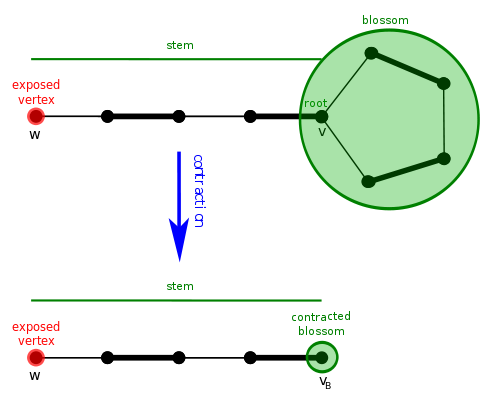
\includegraphics[width=300pt]{blossom_contraction.png}
    \caption{Kontrakce květu, \href{https://en.wikipedia.org/wiki/Blossom_algorithm}{zdroj}}
\end{figure}



\subsection{Datové struktury pro grafové algoritmy}
\label{subsec:data_structures}

Pro implementaci Dijkstrova algoritmu lze použít Fibonacciho haldu
(popis neuvádíme, je poměrně složitý). Pro implementaci Kruskalova
algoritmu používáme strukturu Union Find.

Struktura \textsc{Union Find} ukládá vrcholy do stromů.
Dva vrcholy jsou ve stejné komponentě právě tehdy, když jsou oba
ve stejném stromu, což poznáme pomocí porovnání kořenů (\textsc{Find}).
Spojení komponent probíhá přidáním jednoho stromu k druhému -- to se
řídí podle hodnoty $rank$ každého stromu tak, aby hloubka zůstala nízká.

V \autoref{alg:union_find} proměnnou $self$ používáme ve smyslu jako v
Pythonu. Funkce \textsc{Initialze} je konstruktor.

\begin{algorithm}[H]
\caption{Union Find}
\label{alg:union_find}
\begin{algorithmic}[1]
\Function{Initialize}{$self, V$}
    \State $\forall v \in V : self.parent[v] \gets v, self.rank[v] \gets 0$
\EndFunction

\Function{Find}{$self, v$}
    \While{$self.parent[v] \neq v$}
        \State $v \gets self.parent[v]$
    \EndWhile
    \State \Return $v$
\EndFunction

\Function{Union}{$self, u, v$}
    \State $ru \gets \Call{Find}{u}, rv \gets \Call{Find}{v}$
    \Comment{Najdi kořeny stromů.}
    \If{$ru \neq rv$}
        \If{$self.rank[ru] > self.rank[rv]$}
            \State $self.parent[rv] \gets ru$
        \ElsIf{$self.rank[ru] < self.rank[rv]$}
            \State $self.parent[ru] \gets rv$
        \Else
            \State $self.parent[rv] \gets ru$
            \State $self.rank[ru] \gets self.rank[ru] + 1$
        \EndIf
    \EndIf
\EndFunction

\end{algorithmic}
\end{algorithm}


\subsection{Náhodné grafy a jejich použití}

Ukážeme příklad z~předmětu IA062, kde se pomocí {\em probabilistic
method} dokáže, že nějaká vlastnost v~náhodném grafu platí a z~toho se
potom odvodí náhodnostní algoritmus.

% https://www.corelab.ntua.gr/courses/netalg/presentations/presentations2015/maxcut.pdf

\begin{definition}
    Mějme graf $G$. Problém {\em maximálního řezu} je rozdělit $V$ do
    množin $A, B$ tak, aby $\lvert \{ (u,v) \mid u \in A, v \in B \}
    \rvert$ byla maximální.
\end{definition}

\begin{theorem}
    Pro každý graf $G$ existuje maximální řez velikosti alespoň
    $\lvert E \rvert / 2$.
\end{theorem}

\begin{proof}
    Každý vrchol je s~nezávislou a uniformní pravděpodobností přiřazen
    do jedné z~množin $A, B$. Pravděpodobnost, že hrana je mezi $A, B$
    je tak $1/2$. Podle linearity očekávané hodnoty je velikost řezu
    $\lvert E \rvert / 2$. Z~toho vyplývá, že musí existovat přiřazení
    splňující tvrzení věty\footnote{Tady se právě uplatní myšlenka
    probabilistic method -- aby očekávaná hodnota byla $x$, musí
    existovat nenulová pravděpodobnost, že hodnota je $\geq x$.}.
\end{proof}

\begin{theorem}
    Existuje Las Vegas algoritmus pro hledání řezu velikosti alespoň
    $m/2$.
\end{theorem}

\begin{proof}
    Algoritmus náhodně rozdělí vrcholy do $A, B$, označme velikost řezu
    $s$ a označme
    \[
    p = P(s > \frac{m}{2})
    \]
    Nyní vypočteme
    \[
        \frac{m}{2}
        = \Expect(s)
        = \sum_{i < m/2} i P(s = i)
        + \sum_{i \geq m/2} i P(s = i)
        \leq (1-p)(\frac{m}{2} - 1) + mp
    \]
    což nám dává pravděpodobnost úspěchu
    \[
        p \geq \frac{1}{m/2 + 1}
    \]
    a tedy očekávaný počet opakování náhodného rozdělení je $m/2 + 1$
    (dle věty o očekávané hodnotě geometrického rozdělení).
    Ověření velikosti řezu má složitost nejvýše $m$, celkem tedy máme
    Las Vegas algoritmus s~očekávanou složitostí $\mathcal{O}(m^2)$.
\end{proof}

\subsection{Náhodnostní grafové algoritmy (Kargerův)}

\begin{definition}[Nejmenší řez]
    {\em Řez} $(S,T)$ je rozklad $V$.
    {\em Velikost řezu} $(S,T)$ je
    $w(S,T) = \lvert \{ (u,v) \in E \mid u \in S, v \in T \} \rvert$.
    Řez $(S,T)$ je {\em nejmenší} pokud $w(S,T)$ je nejmenší.
\end{definition}

Problém hledání nejmenšího řezu řeší Kargerův náhodnostní algoritmus.
V grafu vybírá náhodně hrany a kontrahuje je, dokud nezbydou poslední
dva vrcholy. Hrany mezi nimi tvoří vrácený řez.
Kontrakci hrany lze provést v čase $\mathcal{O}(n)$ a provede se jich
$n$, celková složitost je $\mathcal{O}(n^2)$.

\begin{algorithm}
\caption{Kargerův algoritmus}
\label{alg:karger}
\begin{algorithmic}[1]
\Function{Karger}{$G = (V, E)$}
    \While{$\lvert V \rvert \geq 2$}
        \State choose $e \in E$ uniformly at random
        \State contract $e$ in $G$
    \EndWhile
    \State \Return the unique cut of $G$
\EndFunction
\end{algorithmic}
\end{algorithm}

Zbývá analyzovat pravděpodobnost chyby. Nechť $C$ je nějaký zvolený
nejmenší řez s~$k$ hranami. Minimální stupeň v $G$ musí být tedy nejméně
$k$. Pravděpodobnost, že nějaká hrana z~$C$ byla vybrána při první
kontrakci je tedy
\[
    \frac{k}{\lvert E \rvert} \leq \frac{k}{\frac{nk}{2}} = \frac{2}{n}
\]
Při $(i+1)$. kontrakci je to nejvýše $\frac{2}{n-i}$. Pravděpodobnost,
že žádná z~hran $C$ nebyla vybrána (a tedy $C$ je vrácen) je
\[
    \prod_{i = 0}^{n - 3} (1 - \frac{2}{n-i}) =
    \prod_{i = 0}^{n - 3} (\frac{n - i - 2}{n-i}) =
    {n \choose 2}^{-1} =
    \frac{2}{n(n-1)}
\]
Nyní můžeme algoritmus $kn^2$-krát opakovat a získáme následující
horní odhad na pravděpodobnost chyby
(použijeme $1 - x \leq e^{-k}$).
\[
    \big (1 - \frac{2}{n(n-1)} \big )^{kn^2}
    \leq \big (1 - \frac{2}{n^2} \big )^{kn^2}
    \leq \big (e^{-\frac{2}{n^2}} \big )^{kn^2}
    = e^{-2k}
\]
Při $(\log n) n^2$ opakováních tedy dostáváme pravděpodbnost chyby
pouze $\approx \frac{1}{n^2}$. Složitost je $n^4 \log n$.
